
\documentclass[10pt]{article}

\usepackage[utf8]{inputenc}
\usepackage{xcolor}
\usepackage{float}
\usepackage{graphicx}
\usepackage{geometry}
\usepackage{float}
\usepackage[toc,page]{appendix}
\graphicspath{ {./images/} }
\usepackage{hyperref}
\hypersetup{
  colorlinks = true,
  linkcolor = blue,
  citecolor=blue,
  linkbordercolor = {white},
}
\usepackage{fullpage}
\usepackage{fancyvrb}

\frenchspacing

\usepackage{microtype}

\usepackage[english,dutch]{babel}

\usepackage{listings}
% Er zijn talloze parameters ...
\lstdefinestyle{myStyle}{
  belowcaptionskip=1\baselineskip,
  breaklines=true,
  frame=none,
  numbers=left, numberstyle=\tiny, numberfirstline=false, breaklines=true,
  stepnumber=1, tabsize=8,
  basicstyle=\footnotesize\ttfamily,
  keywordstyle=\bfseries\color{blue!40!black},
  commentstyle=\itshape\color{green!40!black},
  identifierstyle=\color{black},
}

\usepackage{caption}
\usepackage{subcaption}

\title{Opdracht 4 \\ \begin{large} Minesweeper\end{large}}
\author{Jenny Vermeltfoort, 3787494}

\begin{document}

\selectlanguage{dutch}
\def\tablename{Tabel}

\maketitle

\section{Uitleg}
Dit verslag beschrijft een applicatie; het spel Minesweeper. De oorsprong van het spel Minesweeper is onzeker, er is
namelijk twijfel tussen verschillende personen. Curt Johnson heeft in 1990 Microsoft Minesweeper ontwikkeld en in 1983
is het spel Mined-out ontwikkeld door Ian Andrew\cite{wik-minsweep}. Minesweeper is geen exact kopie van Mined-out,
maar lijkt er wel zwaar door beinvloed\cite{wik-minout}.

De applicatie bestaat uit een user interface via de Command-line Interface waar de gebruiker verschillende operaties
kan uitvoeren. De applicatie kan ook automatisch worden afgespeeld, zonder enige interactie van de gebruiker. Zie
sectie \ref{sec:gebruik} voor meer informatie.

Wat statistieken van de automatische speler worden in sectie \ref{sec:stat} gepresenteerd.

\section{Gebruik}
\label{sec:gebruik}
Het spel kan gestart worden met het onderstaande commando.
\begin{verbatim}
  $ ./minesweeper --help
  Example: minesweeper --width 10 --height 10 --bomb_count 10
  Example: minesweeper -w 10 -h 10 -b 10 -r ./output.txt -i 1000
  Usage: minesweeper [-w,--width] <num> [-h,--height] <num> 
                     [-b,--bomb_count] <num> 
                     [-r,--robot] <output_path> [-i,--iters] <num>
\end{verbatim}

\begin{enumerate}
  \item de breedte en lengte van het bord configureren.
  \item het aantal bommen configureren.
  \item het programma stoppen,
  \item een vlag plaatsen of verwijderen met 'f' als input.
  \item een vakje openen met spatie als input.
  \item een cursor over het bord verplaatsen met 'h,j,k,l' als inputs.
  \item na een zet, de staat van het vorige bord terughalen, ook wanneer de speler dood is gegaan.
  \item een automatische robot configureren, die random zetten speelt. De resultaten worden geplaatst in de output
        file. De speler kan het aantal iteraties configureren.
\end{enumerate}

\subsection{Valgrind}
Valgrind geeft een weer dat de applicatie geen memmory leaks heeft. Er worden wel een aantal errors gegeven;
voornamelijk problemen onbeschermde pointer, ie pointer dereferences zonder checks. Maar aangezien de applicatie werkt
ga ik hier niet verder op in.

\section{Tijd}
Zie tabel \ref{tab:time} voor de tijd verantwoording.

\begin{table}[H]
  \begin{center}
    \begin{tabular}{ l c }
      Week & Uur \\ \hline
      46   & 4   \\
      47   & 4   \\
      49   & 2   \\
    \end{tabular}

    \caption{Tijd verantwoording}
    \label{tab:time}
  \end{center}
\end{table}

\section{Resultaten}
\label{sec:stat}
De Minesweeper robot is met de volgende configuraties gedraaid:
\begin{itemize}
  \item De verschillende bordmaten: 9x9, 15x15 en 20x20.
  \item Alle maten met verschillende hoeveelheden bommen: 50 of 20 bommen. Dit is bij 9x9,
        60\% en 25\%; bij 15x15, 22\% en 9\%; bij 20x20, 12.5\% en 5\%.
  \item 100.000 potjes per configuratie.
\end{itemize}

Een aantal resultaten zijn zichtbaar in fig. \ref{fig:plots1} en fig. \ref{fig:plots2}. Het is opvallend dat bord maten
vijftien bij vijftien en
twintig bij twintig geen
gewonnen potjes heeft bij vijftig bommen; en met een configuratie van twintig bommen winnen ze beiden binnen 6 zetten,
zie
fig. \ref{fig:plot_15_15_won} en fig. \ref{fig:plot_20_20_won}. Verder duurt een potje maximaal twintig tot
vijfentwintig zetten, te
zien in fig. \ref{fig:plot_9_9_total} en fig. \ref{fig:plot_20_20_total}. De robot verliest bij het negen bij negen
bord ongeveer in 25\%  meer
zetten dan dat het wint. Dit is 22\% bij 20 bommen en 28\% bij 50 bommen, zie fig. \ref{fig:plot_9_9_won} en fig.
\ref{fig:plot_9_9_lost}.

\hfill
\begin{figure}[H]
  \centering
  \begin{subfigure}{.49\textwidth}
    \centering
    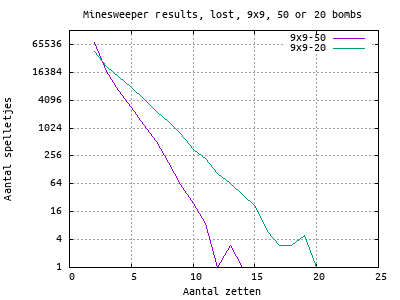
\includegraphics[width=1\linewidth]{plot_9_9_lost}
    \caption{Resultaat verloren, 9x9. }
    \label{fig:plot_9_9_lost}
  \end{subfigure}
  \begin{subfigure}{.49\textwidth}
    \centering
    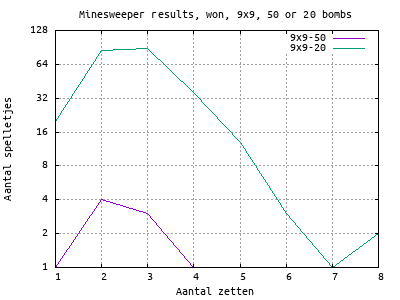
\includegraphics[width=1\linewidth]{plot_9_9_won}
    \caption{Resultaat gewonnen, 9x9. }
    \label{fig:plot_9_9_won}
  \end{subfigure}
  \caption{Resultaten 9x9}
  \label{fig:plots1}
\end{figure}
\begin{figure}[H]
  \begin{subfigure}{.49\textwidth}
    \centering
    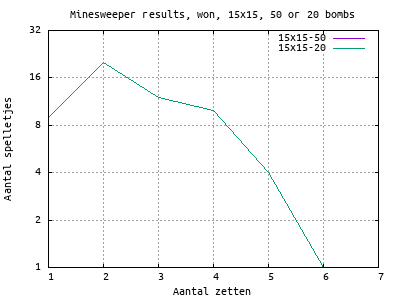
\includegraphics[width=1\linewidth]{plot_15_15_won}
    \caption{Resultaat gewonnen, 15x15. }
    \label{fig:plot_15_15_won}
  \end{subfigure}
  \begin{subfigure}{.49\textwidth}
    \centering
    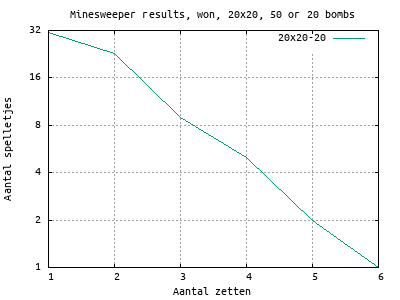
\includegraphics[width=1\linewidth]{plot_20_20_won}
    \caption{Resultaat gewonnen, 20x20. }
    \label{fig:plot_20_20_won}
  \end{subfigure}
  \begin{subfigure}{.49\textwidth}
    \centering
    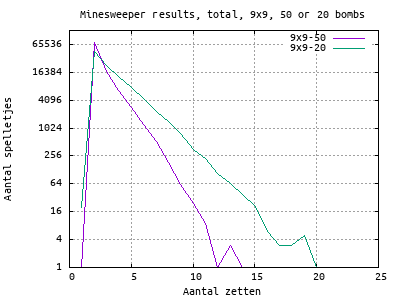
\includegraphics[width=1\linewidth]{plot_9_9_total}
    \caption{Resultaat totaal, 9x9. }
    \label{fig:plot_9_9_total}
  \end{subfigure}
  \begin{subfigure}{.49\textwidth}
    \centering
    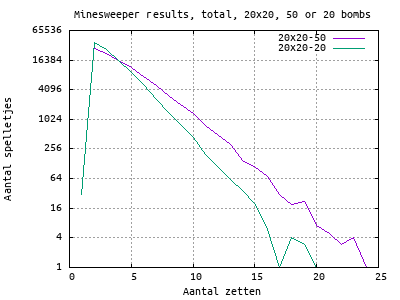
\includegraphics[width=1\linewidth]{plot_20_20_total}
    \caption{Resultaat totaal, 20x20. }
    \label{fig:plot_20_20_total}
  \end{subfigure}
  \caption{Resultaten rest}
  \label{fig:plots2}
\end{figure}

\bibliographystyle{ieeetr}
\bibliography{bibtex.bib}

\newgeometry{left=2cm,bottom=2cm,top=2cm, right=2cm}
\newpage
\begin{appendices}
  \section{Code}\label{sec:code}
  \lstinputlisting[caption=main.cpp,
    language=C++,
    style=myStyle]{../src/main.cpp}

  \lstinputlisting[caption=board.hpp,
    language=C++,
    style=myStyle]{../src/board.hpp}

  \lstinputlisting[caption=board.cpp,
    language=C++,
    style=myStyle]{../src/board.cpp}

  \lstinputlisting[caption=handler.hpp,
    language=C++,
    style=myStyle]{../src/handler.hpp}

  \lstinputlisting[caption=handler.cpp,
    language=C++,
    style=myStyle]{../src/handler.cpp}

  \lstinputlisting[caption=stack.hpp,
    language=C++,
    style=myStyle]{../src/stack.hpp}

  \lstinputlisting[caption=stack.cpp,
    language=C++,
    style=myStyle]{../src/stack.cpp}

  \lstinputlisting[caption=print.hpp,
    language=C++,
    style=myStyle]{../src/print.hpp}

  \lstinputlisting[caption=print.cpp,
    language=C++,
    style=myStyle]{../src/print.cpp}

\end{appendices}

\end{document}